\section{问题一：流失客户画像构建}

\subsection{数据预处理}

原始数据来自题目附件 Telco\_customer\_churn.xlsx，共 7043 条记录、33 个字段，涵盖客户人口统计学信息、账户信息、服务订阅信息和流失标签。

首先对数据进行清洗。剔除 CustomerID、Count、Country 三列：
CustomerID 作为唯一标识，与客户流失情况无关，无泛化预测能力；
Count 恒为 1，方差为 0，对区分客户无贡献；
Country 全部为 United States，无差异性，对模型无额外信息量。

其次，经检查 \texttt{Total Charges} 列为字符串类型。
经 \texttt{pd.to\_numeric}
转换后确认 11 条 \texttt{NaN} 记录。追溯发现这 11 条记录的
\texttt{Tenure Months} 均为 0（新客户尚未产生消费），因此填充为 0，
符合正常业务逻辑。处理后全部 7043 行无缺失值。

为便于后续分析中引用，表 \ref{tab:variable_mapping} 按业务类别
整理了关键变量的中英文名称对照及类别归属。后续分析将围绕表中所列的
时长与费用、合同与支付、服务订阅、人口与家庭四大维度展开。

\begin{table}[H]
    \centering
    \caption{关键变量名称对照表}
    \label{tab:variable_mapping}
    \small
    \begin{tabular}{clll}
        \toprule
        {\heiti 变量类别} & {\heiti 中文名称}
        & {\heiti 原始列名} & {\heiti 说明} \\
        \midrule
        目标变量 & 是否流失 & Churn Value
        & 1=流失, 0=未流失 \\
        \addlinespace
        \multicolumn{4}{l}{\heiti \small （一）时长与费用特征} \\
        数值 & 在网时长 & Tenure Months & 单位：月 \\
        数值 & 月消费金额 & Monthly Charges & 单位：美元 \\
        数值 & 总消费金额 & Total Charges & 单位：美元 \\
        数值 & 客户生命周期价值 & CLTV & Customer Lifetime Value \\
        \addlinespace
        \multicolumn{4}{l}{\heiti \small （二）合同与支付特征} \\
        分类 & 合同类型 & Contract & 月付/一年/两年 \\
        分类 & 支付方式 & Payment Method & 共 4 种 \\
        二分类 & 是否无纸化账单 & Paperless Billing & Yes / No \\
        \addlinespace
        \multicolumn{4}{l}{\heiti \small （三）服务订阅特征} \\
        多分类 & 互联网服务类型 & Internet Service & DSL/Fiber optic/No \\
        二分类 & 在线安全服务 & Online Security & Yes/No/No internet \\
        二分类 & 技术支持服务 & Tech Support & Yes/No/No internet \\
        \addlinespace
        \multicolumn{4}{l}{\heiti \small （四）人口与家庭特征} \\
        二分类 & 是否老年人 & Senior Citizen & Yes / No \\
        二分类 & 是否有配偶 & Partner & Yes / No \\
        二分类 & 是否有家属 & Dependents & Yes / No \\
        \addlinespace
        \multicolumn{4}{l}{\heiti \small （五）其他说明} \\
        文本 & 客户编号 & CustomerID & 无预测价值，已剔除 \\
        数值 & 纬度 & Latitude & 与流失相关系数<0.01 \\
        数值 & 经度 & Longitude & 与流失相关系数<0.01 \\
        \bottomrule
    \end{tabular}
\end{table}

\subsection{流失客户特征探索}

\subsubsection*{整体流失率}

以 Churn Value 为分类依据进行统计，流失客户 $1869$ 人，未流失客户
$5174$ 人，总客户 $7043$ 人，整体流失率为 $26.54\%$，如图
\ref{fig:churn_rate} 所示。

\begin{figure}[H]
    \centering
    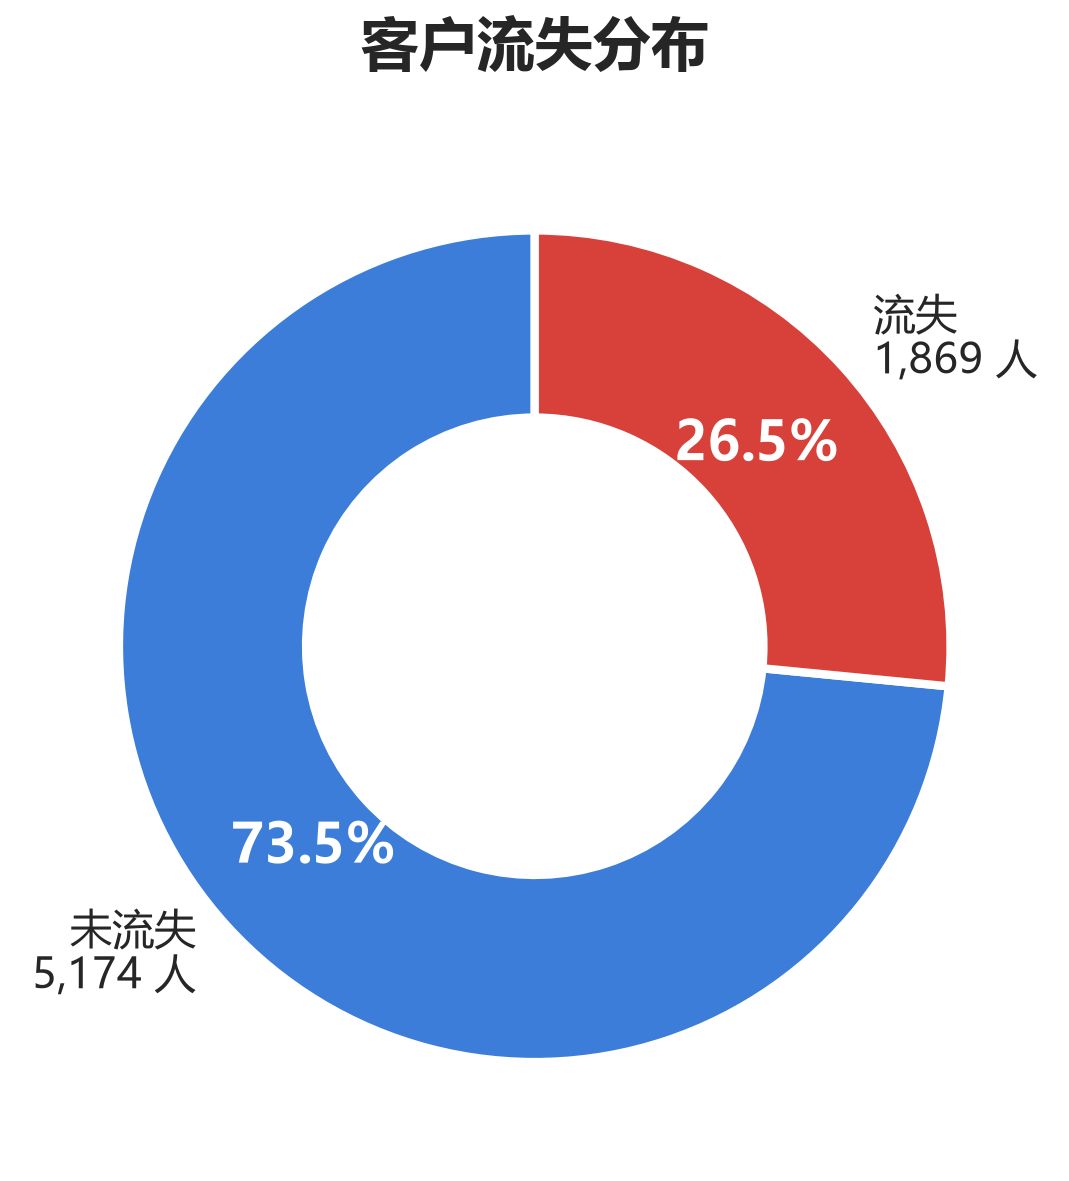
\includegraphics[width=0.5\textwidth]{figures/整体流失率.png}
    \caption{整体流失率环形图}
    \label{fig:churn_rate}
\end{figure}

从分布比例来看，流失与未流失两类样本的比例约为 1:2.8，呈现一定程度的
类别不均衡。这一比例虽然不属严重失衡（如 1:10 以上），但已足以对常规
分类模型的训练过程产生影响——模型倾向于将多数类（未流失）识别得更好
以降低整体损失，而牺牲对少数类（流失）的识别能力。
例如，一个将所有样本都预测为"未流失"的简单模型也能获得 $73.46\%$
的准确率，但这显然不能反映模型在实际业务中的价值。

为此，后续建模中评价指标弃用对类别比例敏感的准确率，
转为采用 AUC 和 F1-score；训练时对逻辑回归设置
\texttt{class\_weight='balanced'} 参数，按类别频数自动调整损失权重，
强化对流失客户的关注。

\subsubsection*{数值特征分布对比}

为考察流失与未流失客户在数值特征上的分布差异，选取在网时长（Tenure Months）、
月消费金额（Monthly Charges）和总消费金额（Total Charges）
三个核心数值特征，分别绘制分组直方图与箱线图，如图 \ref{fig:num_features}
所示。

\begin{figure}[H]
    \centering
    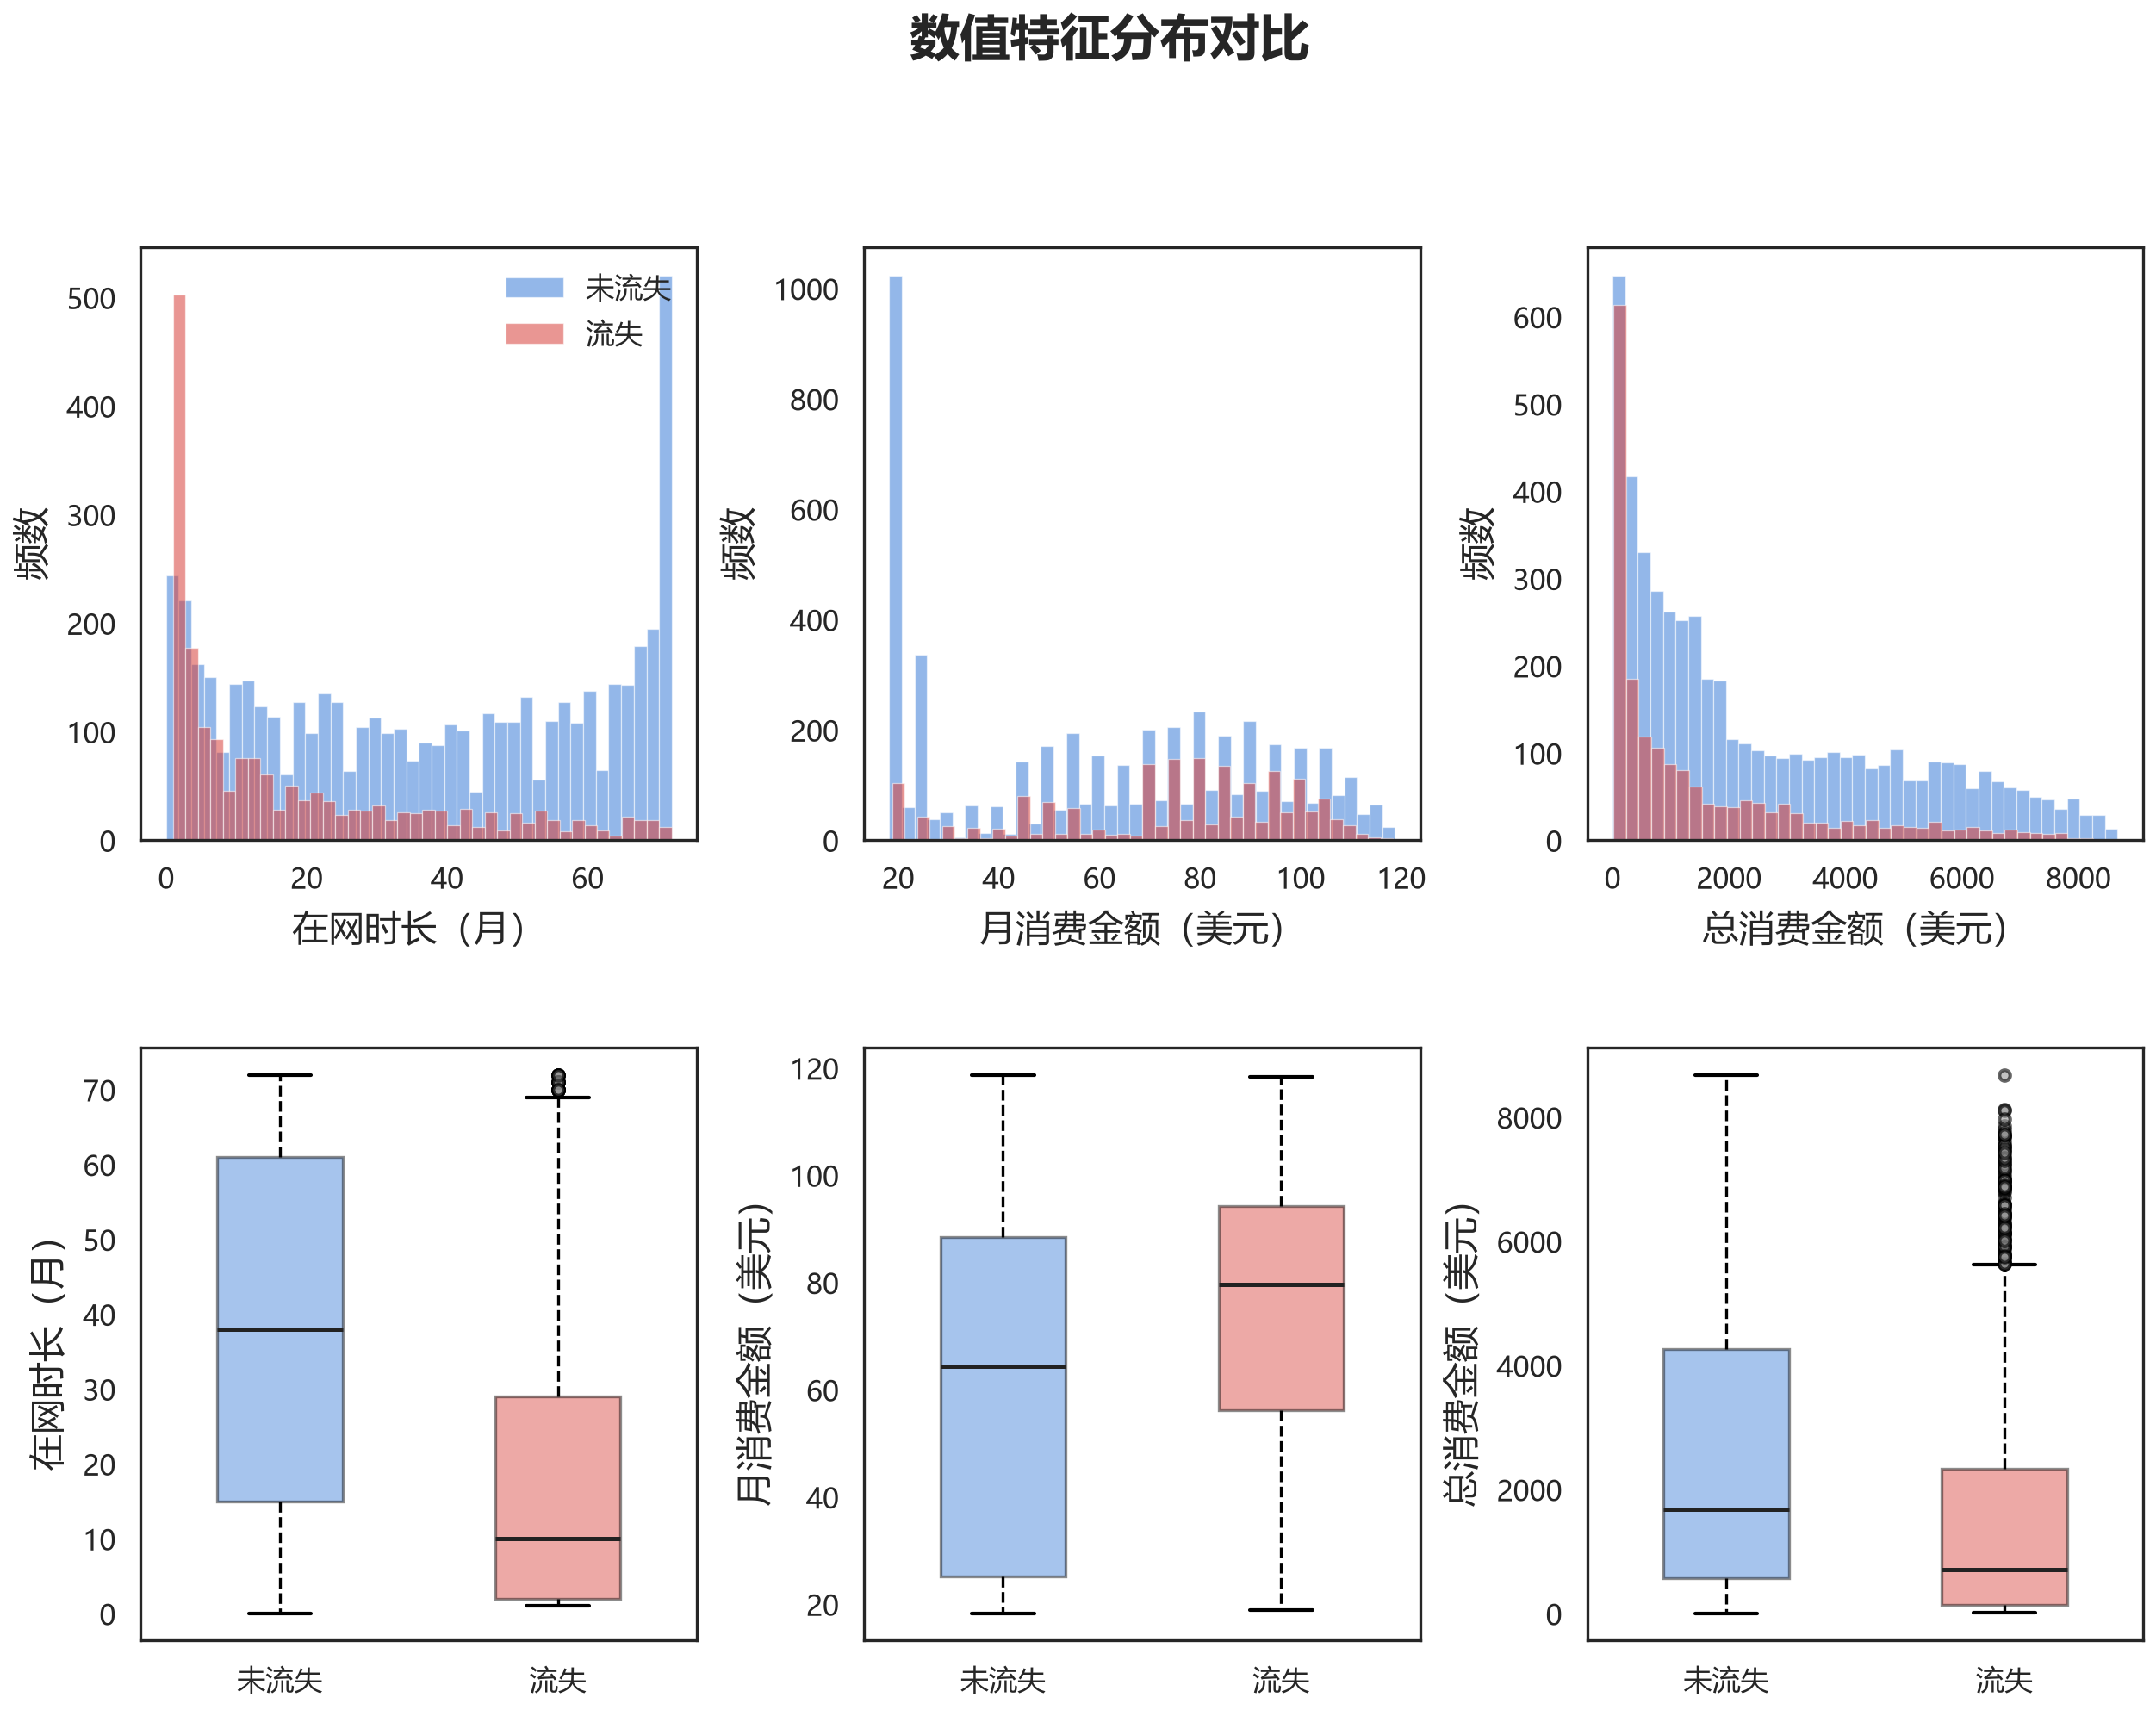
\includegraphics[width=0.85\textwidth]{figures/数值特征分布对比.png}
    \caption{数值特征分布对比图}
    \label{fig:num_features}
\end{figure}

由直方图和箱线图可以观测到以下规律：

\textbf{在网时长：}流失客户的分布高度集中于 0-10 个月的低在网时长区间，
而未流失客户的分布较为均匀，覆盖 0-72 个月的全区间。箱线图显示两组
中位数差距显著，说明在网时长是区分能力最强的数值特征——新客户是流失的
高风险群体。

\textbf{月消费金额：}流失客户的月消费整体偏高，在 70-110 美元的高费区间
聚集密度明显大于未流失客户。高消费客户对价格更为敏感，流失意愿相对更强。

\textbf{总消费金额：}流失客户的总消费明显偏低且呈左偏分布，但该差异主要
源于在网时长短导致的消费积累不足，属于在网时长的间接效应，
其独立区分能力有限。

综合以上分析，在网时长是区分流失与未流失最有效的数值特征。

\subsubsection*{分类特征流失率对比}

为考察分类变量各取值水平下的流失风险差异，选取合同类型、互联网服务
类型、支付方式、是否老年人、是否有配偶、是否有家属、是否开通电话服务、
是否无纸化账单共 8 个分类特征，分别统计各组流失率并绘制柱状图，
如图 \ref{fig:cat_features} 所示。

\begin{figure}[H]
    \centering
    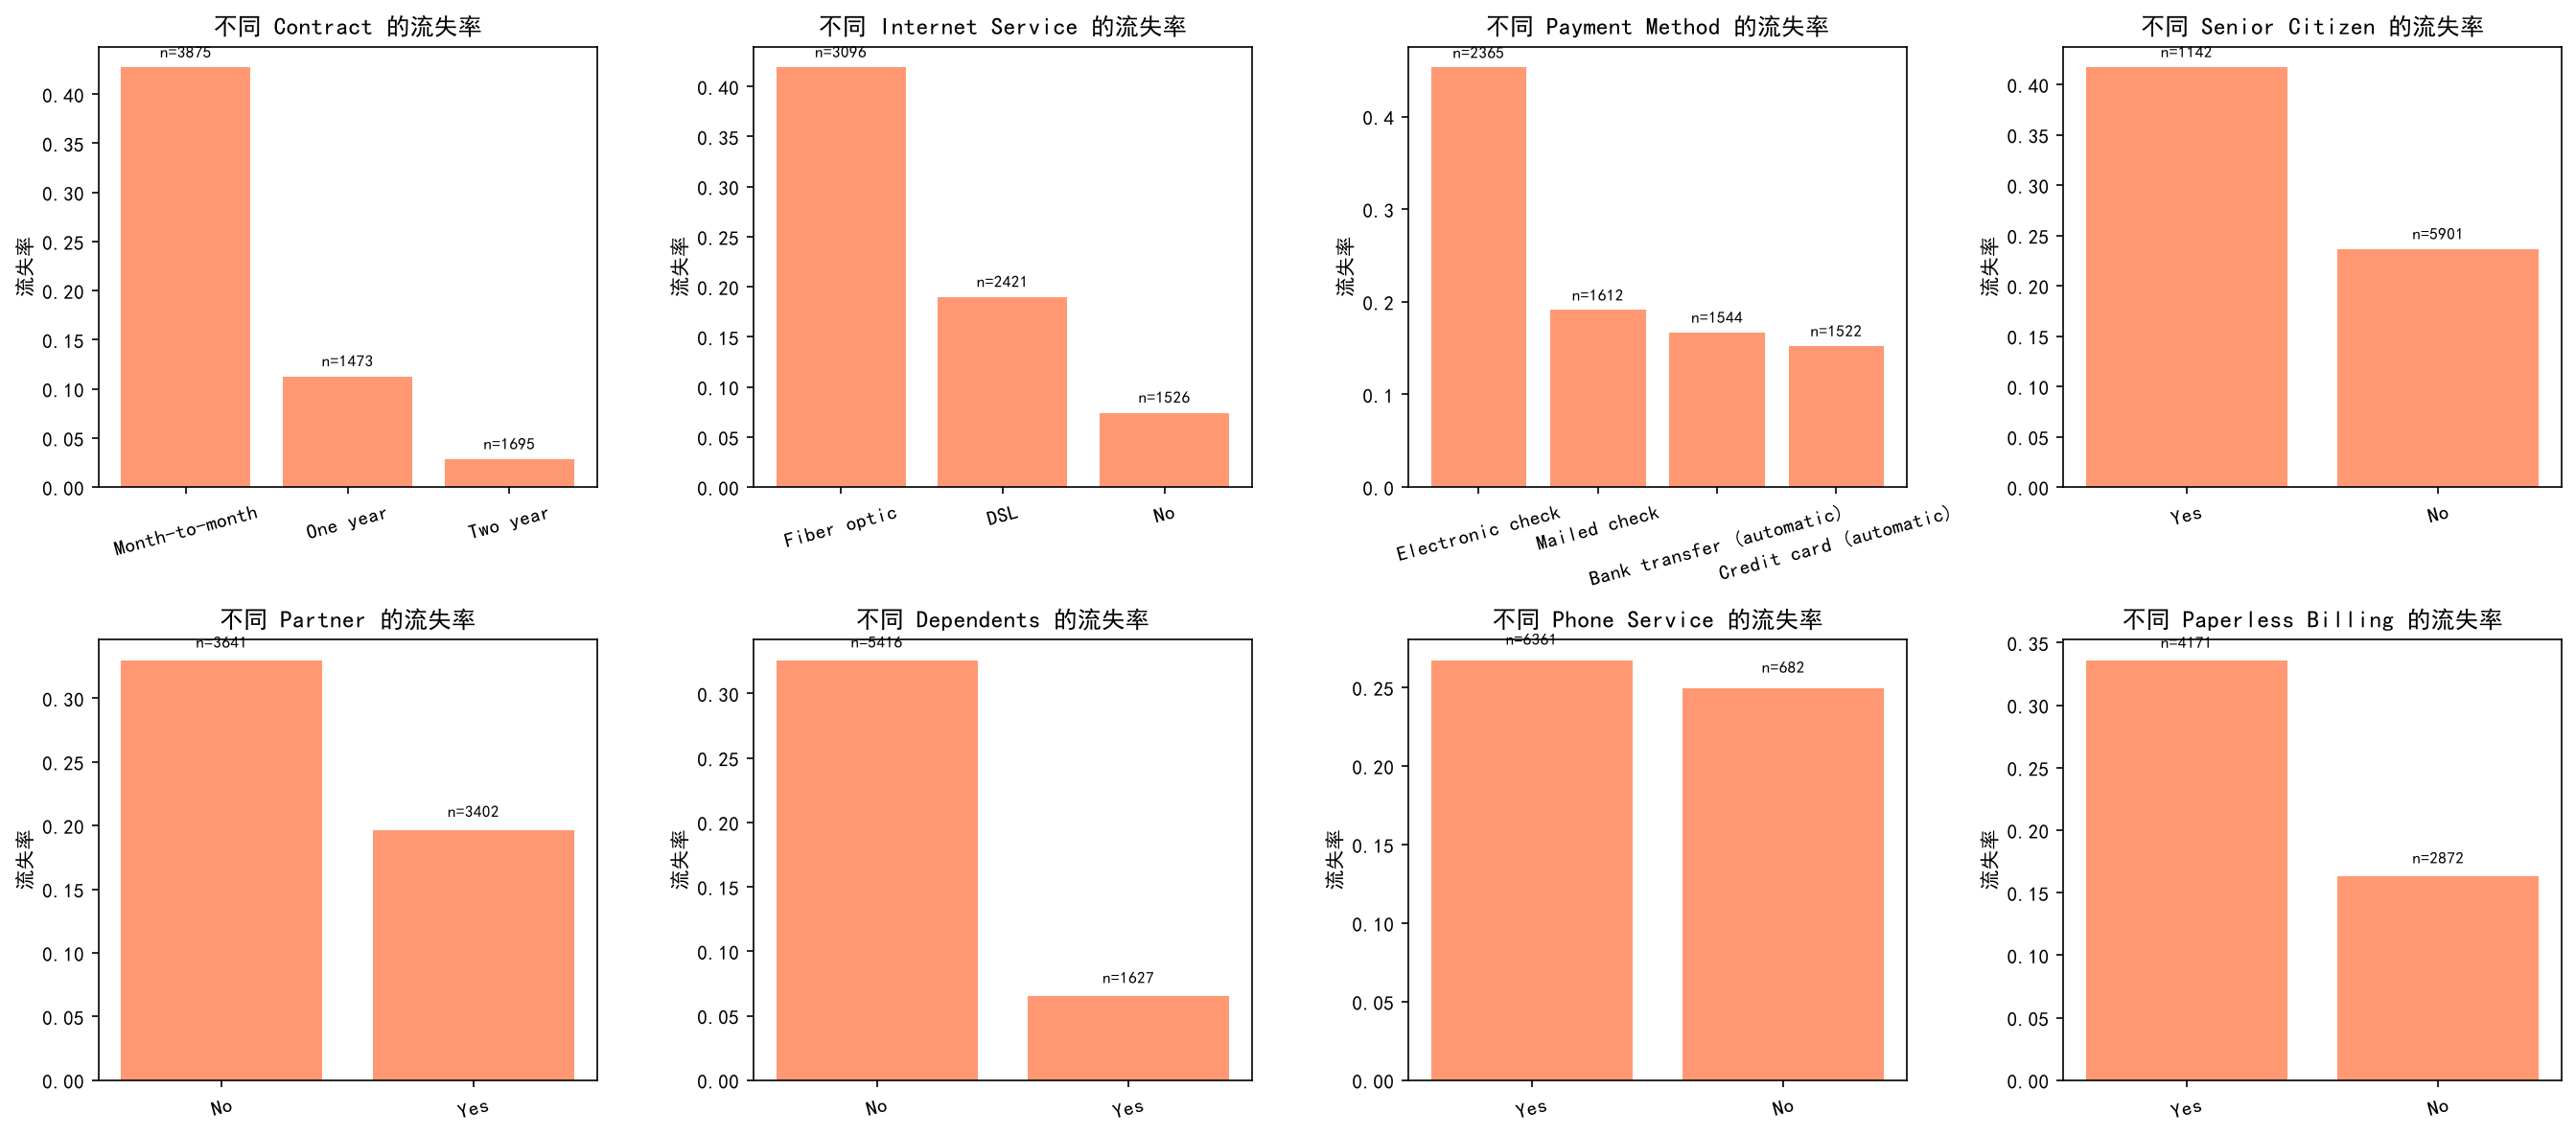
\includegraphics[width=0.85\textwidth]{figures/分类特征流失率对比.png}
    \caption{分类特征流失率对比图}
    \label{fig:cat_features}
\end{figure}

各分类特征的分组流失率如表和图所示，具体分析如下：

\textbf{合同类型（Contract）：}月付合同的流失率超过 40\%，而一年合同
约为 10\%、两年合同约为 3\%。合同期限的差异根本性地改变了客户流失的
转换成本——月付客户可以随时解约，而年付和两年合同的客户通常承担了
提前解约的违约金或已享受合约折扣，转换运营商的意愿显著降低。

\textbf{互联网服务类型（Internet Service）：}光纤客户的流失率显著高于
DSL 客户和无互联网客户，可能与光纤服务的高月费有关——高消费群体对
服务性价比的要求也更高。

\textbf{支付方式（Payment Method）：}电子支票客户的流失率约为 45\%，
而银行自动转账、信用卡自动支付和邮寄支票三种方式的流失率均在
15\%-20\% 之间，表明支付方式与客户属性之间存在一定的关联性。

此外，有配偶或有家属的客户流失率低于独身客户（家庭绑定提高了离网成本），
无纸化账单客户流失率高于纸质账单客户（无纸化账单客户更习惯线上操作，
对运营商的服务切换成本感知较低，更容易比价和更换服务商），而是否老年人
和是否开通电话服务对流失率的影响相对较小。

\subsubsection*{相关性热力图}

采用 Pearson 相关系数衡量各数值特征与流失目标之间的线性关联强度
（取值范围 $[-1, 1]$，绝对值越大线性相关越强）。数值变量的相关系数
矩阵以热力图形式呈现在图 \ref{fig:corr} 中。

\begin{figure}[H]
    \centering
    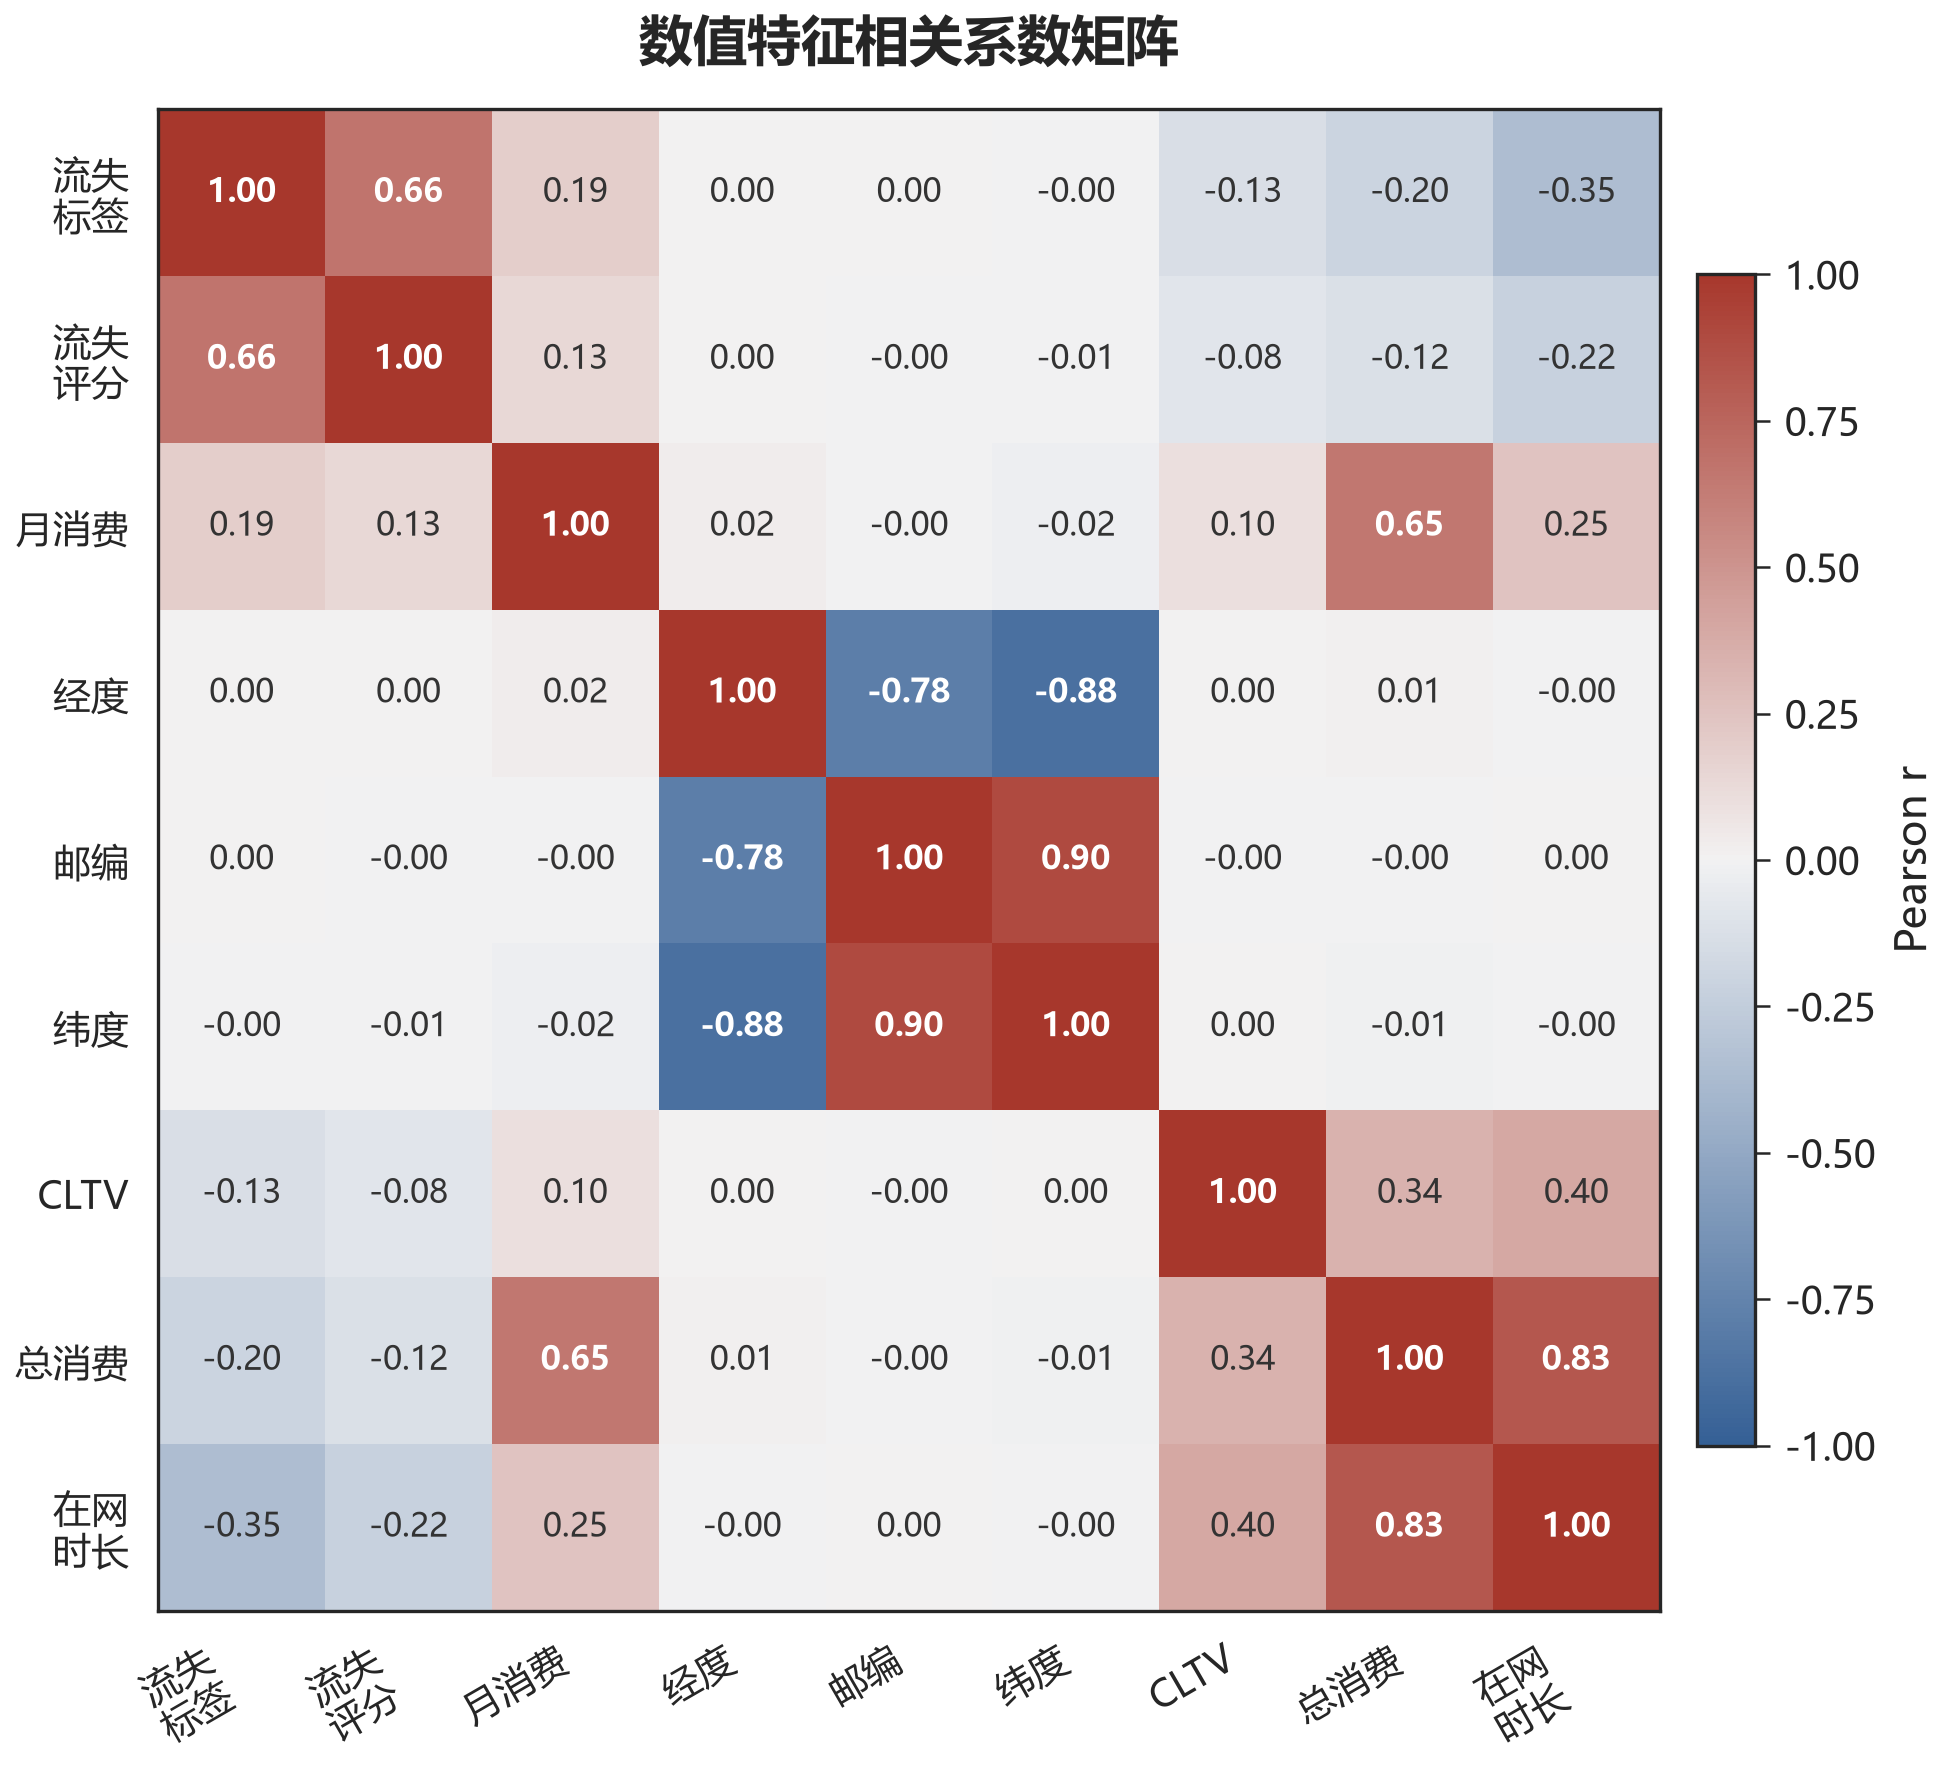
\includegraphics[width=0.75\textwidth]{figures/相关性热力图.png}
    \caption{相关性热力图}
    \label{fig:corr}
\end{figure}

由热力图可见：

\textbf{在网时长：}与流失的相关系数为 $-0.35$，在所有数值特征中
绝对值最大，呈中等程度的负相关——在网时间越长，流失可能性越低，
这与前文分析中"新客户是高危群体"的结论相一致。

\textbf{月消费金额：}与流失的相关系数为 $+0.19$，呈弱正相关——
月消费越高的客户对服务性价比的要求也越高，流失意愿更强，这与分类
特征分析中光纤客户流失率较高的发现互为印证。

\textbf{总消费金额与CLTV：}与流失的相关系数分别为 $-0.20$ 和
$-0.13$，均为弱负相关，方向符合预期。但值得注意的是，在网时长与
总消费之间存在较强的正相关（$r = 0.83$），这是因为在网时间越长累计
消费自然越高，说明两变量存在多重共线性，后续建模中可考虑择一保留。

\textbf{地理特征：}经度、纬度、邮编三个特征与流失的相关系数绝对值
均小于 $0.01$，不具备线性预测价值，说明地理位置与客户的流失决策之间
不存在明显的关联关系。

\subsection{初步结论}

综合上述探索性分析，可从以下维度刻画流失客户的典型特征：
在合同层面，流失客户以月付合同为主，其流失率超过 40\%，
远高于年付和两年合同客户；在在网时长层面，流失客户高度集中在
在网 0-10 个月的新客户群体，在网时长是与流失相关性最强的数值特征
（$r = -0.35$）；在消费层面，流失客户的月消费金额偏高，
高消费群体对服务性价比更为敏感，流失意愿更强；
在家庭层面，无配偶、无家属的独身客户流失率高于有家庭绑定的客户，
前者离网成本更低。

上述发现为下一节分类模型的建立提供了明确的方向：
模型应重点纳入合同类型、在网时长、月消费金额等具有强区分能力的特征变量；
而地理信息（经纬度、邮编）因相关系数绝对值均低于 $0.01$ 可预先剔除，
从而减少模型维度并降低噪声干扰。
